\documentclass[class=book, crop=false, oneside, 12pt]{standalone}
\usepackage[subpreambles=true]{standalone}

\usepackage{../../style}

\graphicspath{{./assets/images/}}

\begin{document}
\chapter{Proprietà dei linguaggi context free}

\section{Proprietà di chiusura}

\subsection*{Chiusura rispetto all'unione}
\begin{lemma}
  La classe dei linguaggi liberi è chiusa rispetto all'operazione di unione d'insiemi.
  \begin{equation*}
    \textrm{Se } \mathcal{L}_1 \land \mathcal{L}_2 \textrm{ sono liberi} \implies \mathcal{L}_1 \cup \mathcal{L}_2 \textrm{ è libero}
  \end{equation*}
\end{lemma}

\begin{proof}
    Siano \(\mathcal{L}_1\) e \(\mathcal{L}_2\) dei linguaggi liberi; questo vuol dire che devono esistere due grammatiche libere, ciascuna delle quali ha generato uno dei due linguaggi. In simboli:

  \begin{equation*}
    \exists \mathcal{G}_1 = (V_1, T_1, S_1, \mathcal{P}_1), \mathcal{G}_2 = (V_2, T_2, S_2, \mathcal{P}_2) : \mathcal{L}_1 = \mathcal{L}(\mathcal{G}_1) \textrm{ e } \mathcal{L}_2 = \mathcal{L}(\mathcal{G}_2)
  \end{equation*}

  Vediamo quindi come costruire una nuova grammatica libera che possa generare l'unione dei due linguaggi generati dalle rispettive grammatiche viste sopra. Consideriamo quindi una nuova grammatica \(\mathcal{G}\), i cui elementi sono così definiti:

  \begin{equation*}
      \mathcal{G} = (V'_1 \cup V'_2 \cup \{S\}, T_1 \cup T_2, S, \mathcal{P}'_1 \cup \mathcal{P}'_2 \cup \{S \rightarrow S'_1 \mid S'_2\})
  \end{equation*}

  \noindent Andiamo a vedere da vicino come sono stati ricavati gli elementi:

  \begin{itemize}
    \item \(V'_1\) e \(V'_2\) si ottengo effettuando un'operazione di \emph{refresh} sui non terminali, in modo da evitare collisioni di nomi (vedremo più avanti come mai quest'operazione è importante), inoltre questo vocabolario è completato con l'introduzione di un nuovo starting symbol;
    \item l'insieme dei terminali è l'unione dei sue insiemi di terminali di \(\mathcal{G}_1\) e \(\mathcal{G}_2\);
    \item \(S\) è il nuovo starting symbol, non presente in \((V'_1 \cup V'_2\), e \(S'_1\) e \(S'_2\) sono di nuovo il refresh degli starting symbol rispettivamente di \(\mathcal{G}_2\) e \(\mathcal{G}_2\);
    \item infine, l'insieme delle produzioni è dato dall'unione tra i refresh delle produzioni delle due grammatiche di partenza  \(\mathcal{G}_1\) e \(\mathcal{G}_2\), unito a una nuova produzione che, dal nuovo starting symbol, produce il resfresh dello starting symbol di una delle due grammatiche di partenza.
  \end{itemize}

  \noindent Questa definizione ci basta per asserire che \(\mathcal{L(G)}\) è libero e \(\mathcal{L(G)} = \mathcal{L}(\mathcal{G}_1)  \cup \mathcal{L}(\mathcal{G}_2) \).

\end{proof}

\begin{osservazione}
  Cerchiamo di capire come mai possiamo essere certi che la grammatica \(\mathcal{G}\), per come l'abbiamo definita, è libera.

  Prendiamo l'insieme delle produzioni di \(\mathcal{G}\); abbiamo già visto come è stato ricavato. Il refreshing va a colpire solamente i nomi dei terminali o non-terminali, non la loro forma, che rimane immutata (\(A \rightarrow \alpha\)). Questa forma è rispettata anche dalle due nuove produzioni aggiunte (\(S \rightarrow S'_1\) e \(S \rightarrow S'_2\)) (e tipo quindi?)

\end{osservazione}

\begin{osservazione}
  Cerchiamo di capire come mai  \(\mathcal{L(G)} = \mathcal{L}(\mathcal{G}_1)  \cup \mathcal{L}(\mathcal{G}_2) \) è valido.
  \begin{itemize}
    \item Consideriamo una stringa \(w \in \mathcal{L(G)}\); questo è vero se e solo se esiste una certa derivazione per ottenerla a partire dallo starting symbol (\(S \implies^* w\)).
    \item Per come abbiamo definito la grammatica \(\mathcal{G}\), il secondo passo della derivazione dev'essere necessariamente il refresh di uno dei due starting symbol delle grammatiche di partenza (\(S \implies S'_1 \implies^* w \lor S \implies S'_2 \implies^* w\));
    \item questo naturalmente è valido se e solo se, a questo punto, la stringa \(w\) può essere derivata in qualche modo a partire da uno degli starting symbol delle grammatiche di partenza (\(S_1 \implies^* w \lor S_2 \implies^* w\)).
    \item Se \(w\) può essere ottenuta attraverso qualche derivazione a partire da \(S_1\) o \(S_2\), allora vuol dire che \(w\) appartiene a uno dei due linguaggi generati dalle nostre due grammatiche di partenza (\(w \in \mathcal{L}(\mathcal{G}_1)  \lor w \in \mathcal{L}(\mathcal{G}_2) \)).
    \item Questo è equivalente ad affermare che \(w\) appartiene all'unione dei due linguaggi (\(w \in \mathcal{L}(\mathcal{G}_1)  \cup \mathcal{L}(\mathcal{G}_2) \)), e ci convince quindi della validità dell'asserto.
  \end{itemize}
\end{osservazione}

\begin{osservazione}
  È semplice convincersi dell'importanza dell'operazione di refreshing. Se consideriamo due grammatiche \(\mathcal{G}_1, \mathcal{G}_2\) con le seguenti produzioni:
  \begin{figure}
    \centering
    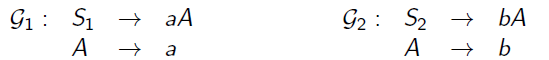
\includegraphics[width=.7\textwidth,keepaspectratio]{why-refresh_1}
  \end{figure}
  \noindent Avremo quindi generati i seguenti linguaggi: \(\mathcal{L}(\mathcal{G}_1)  = \{aa\}\) e \(\mathcal{L}(\mathcal{G}_2)  = \{bb\}\).

  Se non effettuassimo refreshing, Ci troveremo ad avere una nuova grammatica con le seguenti produzioni:
  \begin{figure}
    \centering
    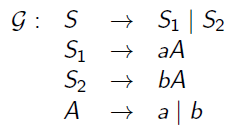
\includegraphics[width=.3\textwidth,keepaspectratio]{why-refresh_2}
  \end{figure}
  \noindent Il linguaggio prodotto da questa nuova grammatica sarebbe diverso da quello dato dall'unione delle due grammatiche di partenza, poiché avremmo \(\mathcal{L(G)} = \{aa, ab, ba, bb\} \neq \mathcal{L}(\mathcal{G}_1)  \cup \mathcal{L}(\mathcal{G}_2) \).

  Con un'opportuno resfreshing otteniamo invece:
  \begin{figure}
    \centering
    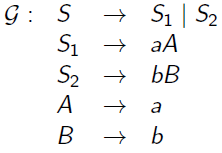
\includegraphics[width=.3\textwidth,keepaspectratio]{why-refresh_3}
  \end{figure}
  Questo insieme di produzioni garantisce che la grammatica generi il linguaggio desiderato.
\end{osservazione}

\subsection*{Chiusura rispetto alla concatenazione}

\begin{lemma}
  La classe dei linguaggi liberi è chiusa rispetto all'operazione di concatenazione.

  \begin{equation*}
    \textrm{Se } \mathcal{L}_1 \land \mathcal{L}_2 \textrm{ sono liberi} \implies \{w_1w_2 \mid w_1 \in \mathcal{L}_1 \land w_2 \in \mathcal{L}_2\} \textrm{ è un linguaggio libero.}
  \end{equation*}

\end{lemma}

\begin{proof}
  % Consideriamo due linguaggi liberi \(\mathcal{L}_1\) e \(\mathcal{L}_2\);
  La dimostrazione sembra assolutamente uguale a quella del lemma della chiusura all'unione, sono confuso ma domani cercherò di chiarire.
\end{proof}

\subsection*{Chiusura rispetto all'interezione}

\begin{lemma}
  La classe dei linguaggi liberi è chiusa rispetto all'operazione d'intersezione.
\end{lemma}

\begin{proof}
  La dimostrazione è per contraddizione, è sufficiente trovare due linguaggi liberi la cui intersezione non è libera.

  Si considerino, ad esempio, due linguaggi \(\mathcal{L}_1\) e \(\mathcal{L}_2\), definiti come segue:
  \begin{align*}
      \mathcal{L}_1 = \{a^n b^n c^j \mid n, j > 0 \} \\
      \mathcal{L}_2 = \{a^j b^n c^n \mid n, j > 0 \}
  \end{align*}

  \noindent Il linguaggio generato dalla loro intersezione è il seguente:

  \begin{align*}
    \mathcal{L}_1 \cap \mathcal{L}_2 = \{ a^n b^n c^n \mid n > 0 \}
  \end{align*}

  \noindent Questo linguaggio non è libero, e provarlo è molto semplice (si veda \ref{ex-freeNotfree_1}).

\end{proof}

\section{Chomsky Normal Form}
\paragraph{Definizione}
Una grammatica libera \(\mathcal{G} = (V, T, S, \mathcal{P})\) è in \emph{Chomsky Normal Form} se e solo se:
\begin{itemize}
  \item non ha alcuna \(\varepsilon\)-produzione, al massimo \(S \rightarrow \varepsilon\);
  \item tutte le sue non \(\varepsilon\)-produzioni  una tra le due seguenti forme:
  \begin{itemize}
    \item \(A \rightarrow a\)
    \item \(A \rightarrow BC\)
  \end{itemize}
  in cui sia \(B\) sia \(C\) sono diversi da \(S\).
\end{itemize}

\begin{lemma}
  Sia \(\mathcal{G}\) una grammatica libera; allora esiste una certa grammatica \(\mathcal{G'}\) in Chomsky Normal Form tale che \(\mathcal{L(G)} = \mathcal{L(G')}\).
\end{lemma}

\noindent La dimostrazione del lemma è lasciata per esercizio.

\section{Come epurare le grammatiche libere}
Esiste un teorema che ci permette di fare pulizia etnica sui linguaggi.
\begin{theorem}
  Consideriamo un linguaggio libero \(\mathcal{L}\); allora esiste una grammatica libera \(\mathcal{G}\) tale che \(\mathcal{L(G)} = \mathcal{L}\setminus\varepsilon\) e tale da:
  \begin{itemize}
    \item non avere alcuna \(\varepsilon\)-produzione, ovvero produzioni di forma \(A \rightarrow \varepsilon\);
    \item non avere alcuna produzione d'unità (\emph{unit production}), ovvero produzione di forma \(A \rightarrow B\);
    \item non avere alcun non-terminale non utile, ovvero non-terminali che non appaiono mai in alcuna derivazione di qualche stringa di terminale.
  \end{itemize}
\end{theorem}

Le grammatiche che possiedono queste caratteristiche sono più sintetici e generano linguaggi equivalenti a livello espressivo, ma più puliti; ad esempio, non c'è alcun bisogno di avere molti non-terminali che abbiano una produzione in \(\varepsilon\) e, qualora richiesto, la produzione \(S \rightarrow \varepsilon\) sarebbe sufficiente allo scopo (da approfondire).

Non è nostro interesse entrare nel dettaglio degli algoritmi per effettuare questa pulizia, poiché dimostrarne la correttezza richiederebbe un considerevole impegno. Andremo però ad analizzare come possiamo, se non altro,  eliminare le \(\varepsilon\)-produzioni.

\subsection{Come eliminare le \(\varepsilon\)-produzioni}
Per eliminare le \(\varepsilon\)-produzioni bisogna procedere ad individuare i non-terminali \emph{annullabili}, ovvero quei non-terminali che, con qualche derivazione, producono la parola vuota (\(A : A \rightarrow^* \varepsilon\)). Si può procedere ricorsivamente:
\begin{itemize}
  \item base: se la grammatica comprende una produzione della forma \(A \rightarrow \varepsilon\), allora quel non-terminale \(A\) è annullabile;
  \item iterazione: se la grammatica comprende una produzione della forma \(A \rightarrow Y_1Y_2 \ldots Y_n\) e i non terminali \(Y_1, Y_2, \ldots, Y_3\) sono tutti annullabili, allora anche \(A\) è annullabile.
\end{itemize}
A questo punto, andiamo a sostituire ogni produzione della forma \(A \rightarrow Y_1Y_2 \ldots Y_n\) con una famiglia di produzioni dove ogni combinazione di \(Y_i\) annullabili è rimossa dal body della produzione. Se tutti gli \(Y_i\) sono annullabili, non bisogna includere nella famiglia risultante la produzione \(A \rightarrow \varepsilon\). Quindi, si elimina ogni produzione \(A \rightarrow \varepsilon\).

\paragraph{Esempio di applicazione}
Andiamo a vedere un esempio considerando la seguente grammatica:
%
% \begin{figure}
%   \centering
%   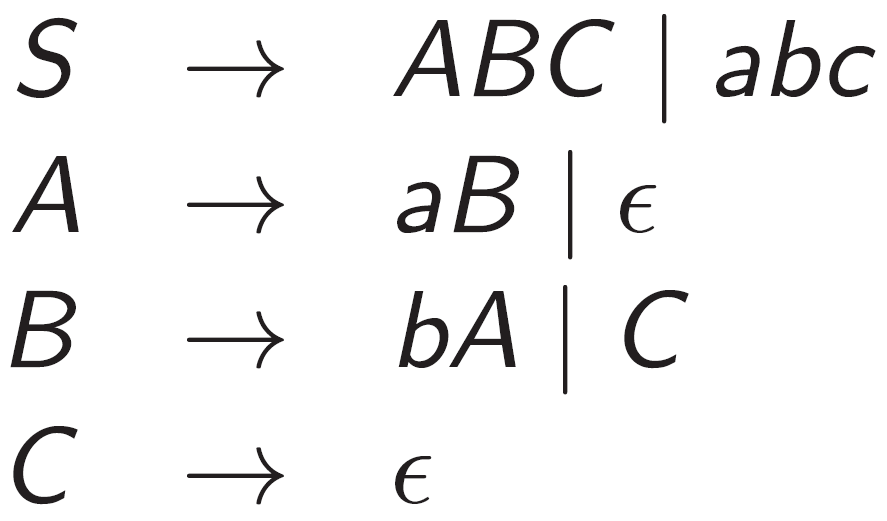
\includegraphics[width=.3\textwidth,keepaspectratio]{ex-th-1-3-1_1}
% \end{figure}

\begin{align*}
  S\; & \to\; ABC\; \mid abc \\
  A\; & \to\; aB\; \mid \varepsilon \\
  B\; & \to\; bA\; \mid C \\
  C\; & \to\; \varepsilon
\end{align*}

Osserviamo subito che sia \(A\) sia \(C\) hanno una produzione che conduce a \(\varepsilon\), pertanto sono annullabili; allo stesso modo, \(B\) è annullabile attraverso \(C\) e \(S\) è annullabile attraverso \(A, b\) e \(C\). Con le operazioni che abbiamo illustrato poc'anzi, la grammatica che otteniamo è la seguente:

% \begin{figure}
%   \centering
%   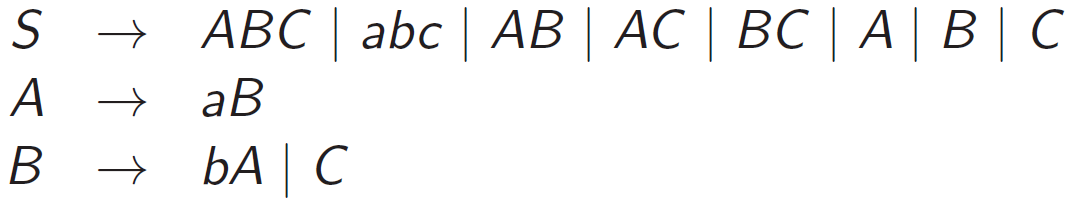
\includegraphics[width=.3\textwidth,keepaspectratio]{ex-th-1-3-1_2}
% \end{figure}

\begin{align*}
  S\; & \to\; ABC\; \mid abc\; \mid AB\; \mid AC\; \mid AC\; \mid BC\; \mid A\; \mid B\; \mid C \\
  A\; & \to \; aB \\
  B\; & \to\; bA\; \mid C
\end{align*}

Si noti che, in questa grammatica, il non-letterale \(C\) è non utile.

\section{Pumping lemma for free languages}

\subsection{Definizione e formulazione}

Si segua lentamente formulazione e dimostrazione per questo tanto articolato quanto importante lemma.

\begin{lemma}
  Consideriamo un linguaggio libero \(\mathcal{L}\), allora:
  \begin{itemize}
    \item \(\exists p \in \mathbb{N}^+\) tale che
    \item \(\forall z \in \mathcal{L} : |z| > p\), allora
    \item \(\exists u, v, w, x, y\) tale che:
    \begin{itemize}
      \item \(z = uvwxy \textrm{ } \land\)
      \item \(|vwx| \leq p \textrm{ } \land\)
      \item \(|vx| > 0 \textrm{ }\land\)
      \item \(\forall i \in \mathbb{N}.uv^iwx^iy \in \mathcal{L}\)
    \end{itemize}
  \end{itemize}
\end{lemma}

\begin{proof}
  Partiamo considerando un linguaggio libero \(\mathcal{L}\) che non comprende la parola vuota (\(\varepsilon \notin \mathcal{L}\)); sappiamo quindi che deve esistere una grammatica libera "epurata" \(\mathcal{G}\) che generi il linguaggio \(\mathcal{L}\) (\(\mathcal{L} = \mathcal{L(G)}\)).

  Osserviamo che, per ogni possibile albero di derivazione, ogni cammino dalla radice a un terminale attraversa tanti non-terminali quanto il valore della lunghezza del cammino stesso. Ad esempio, la lunghezza del cammino \(\langle S, B_1, B_2, \ldots, B_{k-1}, a \rangle\) è \(k\), così come il numero di non-terminali attraversati.

  Adesso definimo \(p\) come la lunghezza della più lunga parola derivabile con degli alberi di derivazione, e che inoltre sia tale che i suoi camini, a partire dalla radice, siano lunghi al più come il numero di non-terminali di \(\mathcal{G}\). Consideriamo quindi anche una parola \(z \in \mathcal{L}\), più lunga di \(p\) (\(|z| > p\)). Possiamo quindi essere sicuri che esiste un albero di derivazione per \(z\) che possiede almeno un cammino la cui lunghezza è strettamente maggiore del numero di non-terminali, poiché \(|z| >p\).

  Adesso, per un qualche albero di derivazione, andiamo a considerare la più profonda coppia di occorrenze dello stesso non-terminale lungo un qualche cammino; con più profonda coppia di occerrenze intendiamo la coppia composta dalla più lontana e dalla seconda più lontana occorrenza dalla radice di uno stesso non terminale.

  Andiamo a visualizzare la situazione attraverso un albero di derivazione, considerando le due occorrenze di un non-terminale \(A\).

  \begin{figure}
    \centering
    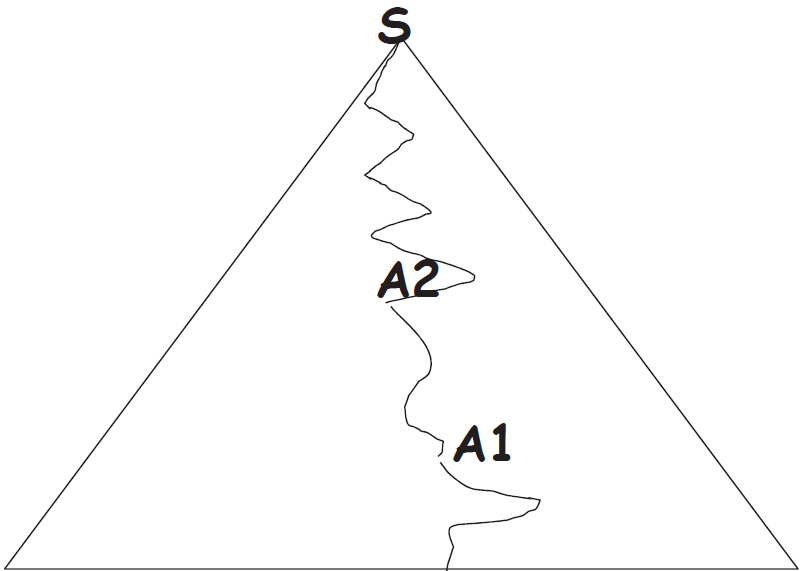
\includegraphics[width=.25\textwidth,keepaspectratio]{pl-proof_1}
  \end{figure}

  Possiamo dire, nelle due occorrenze di \(A\), sono radicati due sottoalberi distinti, che noi qui rappresenteremo colorati di verde e porpora. La parola \(z\) può quindi essere "spacchettata" in cinque sottoparole, come illustrato di seguito.

  \begin{figure}
    \centering
    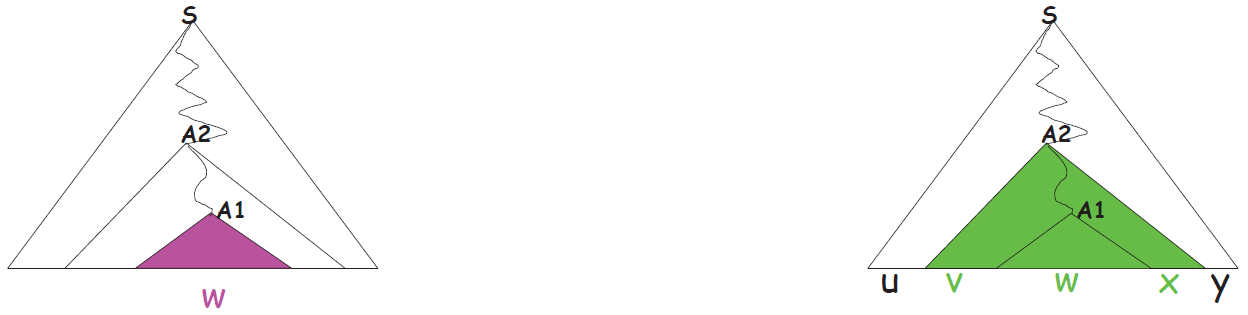
\includegraphics[width=.8\textwidth,keepaspectratio]{pl-proof_2}
  \end{figure}

  Dal momento che \(A_1\) e \(A_2\) sono occorrenze di uno stesso non-terminale, condividono la medesima famiglia di produzioni. Questo fatto è notevole: se, a partire da \(A_2\), siamo riusciti a trovare una qualche sequenza di derivazioni tale da essere arrivati a \(A_1\), allora con la stessa sequenza possiamo trovare una nuova occorrenza di \(A\), il che ci rende ragionevolmente certi che possiamo generare un numero arbitrario di sottostringhe \(v, x\) di \(z\).

  \begin{figure}[H]
    \centering
    \begin{minipage}{0.25\textwidth}
      \centering
      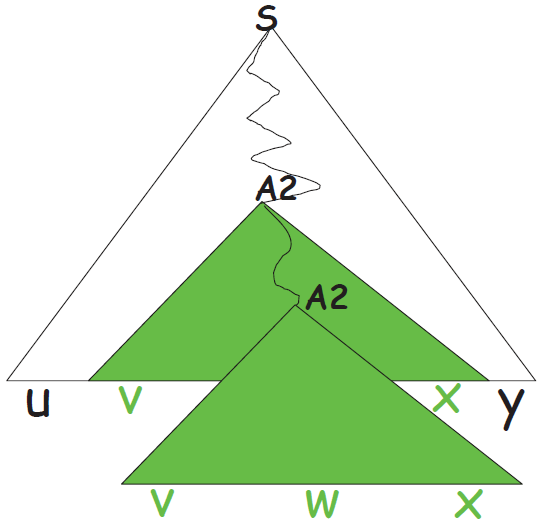
\includegraphics[width=\textwidth,keepaspectratio]{pl-proof_3}
    \end{minipage}
     \hfill
    \begin{minipage}{0.25\textwidth}
      \centering
      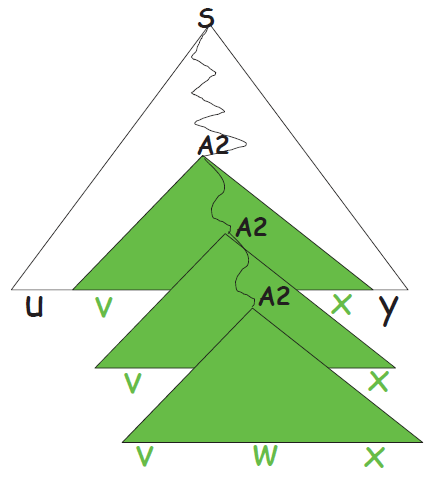
\includegraphics[width=\textwidth,keepaspectratio]{pl-proof_4}
    \end{minipage}
  \end{figure}


  Allo stesso modo sappiamo che, se a partire da \(A_1\) possiamo otteniamo un sottoalbero di derivazioni \(w\), questo stesso sottoalbero può essere ottenuto a partire da \(A_2\).

  \begin{figure}
    \centering
    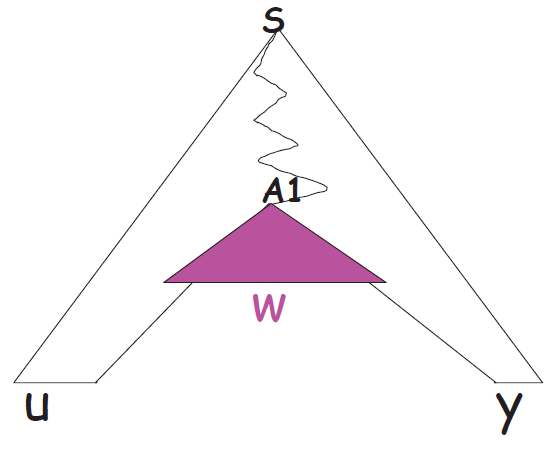
\includegraphics[width=.25\textwidth,keepaspectratio]{pl-proof_5}
  \end{figure}

  Queste affermazioni possono essere riassunte, per l'appunto, nella formula:

  \begin{equation*}
    \forall i \in \mathbb{N}.uv^iwx^iy \in \mathcal{L}
  \end{equation*}

  Ulteriori considerazioni:
   \begin{itemize}
     \item per come abbiamo scelto le occorrenze di \(A\), la profondità del sottoalbero radicato in \(A_2\) è minore del numero di non-terminali presenti nella grammatica considerata, da cui, per definizione stessa del valore \(p\), \(|vwx| < p\);
     \item la grammatica \(\mathcal{G}\) che genera il linguaggio che stiamo considerando è ripulita, per cui nelle derivazioni di forma \(A \implies^* \alpha A \beta\), almeno uno dei due simboli \(\alpha, \beta\) deve fornire uno ulteriore; questo ci permette di affermare che \(|vx| > 0\).
   \end{itemize}

   \paragraph{Dimostrazione se \(\varepsilon \in \mathcal{L}\)}
   La dimostrazione che abbiamo appena concluso è relativa a linguaggi privi di parola vuota, ma con un attimo di cura nell'impostazione possiamo estenderla anche ai linguaggi che comprendono \(\varepsilon\).

   Considerando un linguaggio \(\mathcal{L}\) che comprenda \(\varepsilon\), partiamo ricavando una grammatica \(\mathcal{G} = (V, T, S, \mathcal{P})\) che generi \(\mathcal{L} \setminus \{\varepsilon\}\). A questo punto definiamo una seconda nuova grammatica \(\mathcal{G}'\), in cui andiamo semplicemente ad aggiungere un nuovo starting symbol assieme a due produzioni: una che punti verso lo starting symbol della precedente grammatica, e una seconda che generi invece \(\varepsilon\). Formalmente:

   \begin{equation*}
     \mathcal{G}' = (V, T, S', \mathcal{P} \cup \{ S' \rightarrow S, S' \rightarrow \varepsilon \})
   \end{equation*}

   In questo modo abbiamo che \(\mathcal{L} = \mathcal{L(G')}\) e possiamo procedere analogamente a prima

\end{proof}

\subsection{Applicazioni}

	Qui passiamo alle applicazioni del \emph{Pumping Lemma}. In particolare può essere utilizzato per provare che un linguaggio \(\mathcal{L}\) non è libero.

	In generale, da una implicazione logica del tipo \(A \implies B\), è possibile ottenere la negazione \(!A \implies !B\). Nel nostro caso, da \(\mathcal{L}\) libero \(\implies\) Tesi del \emph{Pumping Lemma}, abbiamo \(Not\) tesi del \emph{Pumping Lemma} \(\implies\) \(\mathcal{L}\) \(Not\) libero.
	La negazione della tesi del \emph{Pumping Lemma} è la seguente:

	\begin{itemize}
		\item \(\forall p \in \mathbb{N}^+\) tale che
		\item \(\exists z \in \mathcal{L} : |z| > p\), allora
		\item \(\forall u, v, w, x, y\) tale che:

		\begin{itemize}
			\item \(z = uvwxy \textrm{ } \land\)
			\item \(|vwx| \leq p \textrm{ } \land\)
			\item \(|vx| > 0 \textrm{ }\land\)
			\item \(\exists i \in \mathbb{N}.uv^iwx^iy \not\in \mathcal{L}\)
		\end{itemize}

	\end{itemize}

	Lasciamo al lettore immaginare gli altri modi in cui è possibile riscrivere la negazione della tesi del \emph{Pumping Lemma} applicando le basi di algebra booleana.
	Passiamo dunque ad esempi pratici.
	ES 1
	Sia \(\mathcal{G}\) così definito
	\(S \rightarrow aSb \ abc\)
	\(cB \rightarrow Bc\)
	\(bB \rightarrow bb\)
	ci chiediamo dunque se \(\mathcal{G}\) è \emph{context dependent} o \emph{free}. Ovviamente è \emph{context dependent}.
	Ci chiediamo quale sia il linguaggio generato da \(\mathcal{G}\), \(\mathcal{L(G)}\) ed è \({a^n b^n b^n | n>0}\)
	Ci chiediamo infine se il linguaggio \(\mathcal{L(G)}\) sia o meno un linguaggio libero. Per farlo possiamo semplicemente utilizzare la negazione del \emph{Pumping Lemma} per dimostrare che \(\mathcal{L(G)}\) non è libero.

	Sia \( p \in N^+\) un numero intero arbitrario
	Possiamo prendere un numero \(z=a^pb^pc^p \in \mathcal{L}\) che soddisfa la condizione \(|z|\leq p\)
	Quindi possiamo prendere qualsiasi decomposizione di \(z = uvwxy, |vwx|\leq p |vx|>0\).
	Sappiamo che la parola \(z\) è composta in questo modo. \(\underbrace{aa...a}_\text{\emph{p}}\underbrace{bb...b}_\text{\emph{p}}\underbrace{cc...c}_\text{\emph{p}}\).
	La sottostringa \(vwx\) deve essere sicuramente in una di queste possibili posizioni
	\(a\underbrace{a...a}_\text{\emph{vwx}}
	a\underbrace{a...abb...b}_\text{\emph{vwx}}
	b\underbrace{b...b}_\text{\emph{vwx}}
	b\underbrace{b...bc...c}_\text{\emph{vwx}}
	c\underbrace{c...c}_\text{\emph{vwx}}c\)
	da cui abbiamo che qualsiasi sia la posizione di \(vwx\) all'interno della parola \(z\) è possibile costruire una parola con un numero non bilanciato di \(a,b,c\) semplicemente ponendo \(v^i,x^i,i=0\)
	Dunque troviamo una parola che non appartiene al linguaggio. Se il linguaggio fosse libero, tutte le parole costruite in questa maniera dovrebbero appartenere al linguaggio. Dunque il linguaggio non è
	\emph{free}
	Passiamo dunque ad un altro esempio riprendendo l'esercizio lasciato per casa a suo tempo
	ES 2

	\(S \rightarrow CD \)
	\(C \rightarrow aCA | bCB \)
	\(AD \rightarrow aD \)
	\(BD \rightarrow bD \)
	\(Aa \rightarrow aA \)
	\(Ab \rightarrow bA \)
	\(Ba \rightarrow aB \)
	\(Bb \rightarrow bB \)
	\(C \rightarrow \epsilon \)
	\(D \rightarrow \epsilon \)

	Si verifica facilmente che il linguaggio generato da tale grammatica è \(\mathcal{L(G)} =\{ww | w\in\{a,b\}^*\}\)
	Ci chiediamo allore se tale linguaggio sia libero o meno
	Un lettore naive potrebbe essere portato ad applicare la proprietà di chiusura dei linguaggi liberi rispetto alla operazione di concatenazione per dimostrare che suddetto linguaggio sia libero, in quanto sappiamo che \(\mathcal{L'(G)} =\{w | w\in\{a,b\}^*\}\) è un linguaggio libero. Tuttavia l'operazione di concatenazione non rispetta la proprietà di palindromia di \(\mathcal{L}\).
	È infatti semplice provare che \(\mathcal{L}\) non è libero
	DIM
	Sia \(\mathcal{L}\) libero
	sia \(z=a^pb^pa^pb^p, z\in \mathcal{L}, z=uvwxy, |vwx|\leq p \)
	Per esempio supponiamo sia \(|vwx|=b^p\), allora ic è facile prendere \(uv^0wx^0y\) e verificare che questo non può avere la forma \(a^pb^pa^pb^p\)
	Dunque abbiamo trovato un elemento che contraddice il \emph{Pumping Lemma} e dunque l'ipotesi iniziale non è valida, ovvero \(\mathcal{L}\) non è \emph{free}



\section{...}

\section{Alcuni esercizi che contestualizzerò meglio più avanti}
\subsection*{Esercizio 1 - I seguenti linguaggi sono liberi?}

\begin{table}[H]
	\centering
	\subimport{assets/tables/}{ex-freeNotFree_1.tex}
    \caption{Esercizio 1}
    \label{ex-freeNotFree_1}
\end{table}

\paragraph{Spiegazione \ref{ex-freeNotFree_1}}
Questo linguaggio non è libero perché non è possibile trovare una grammatica che sia libera e che lo generi (c'è anche una qualche prova? Pumping lemma maybe?)

\begin{table}[H]
	\centering
	\subimport{assets/tables/}{ex-freeNotFree_2.tex}
    \caption{Esercizio 2}
    \label{ex-freeNotFree_2}
\end{table}

\paragraph{Spiegazione \ref{ex-freeNotFree_2}}
Per provare che questo linguaggio è libero possiamo sfruttare la chiusura dei linguaggi liberi rispetto alla concatenazione. È semplice trovare una grammatica libera che generi il linguaggio \( \{ a^nb^n \mid n > 0 \} \), come ad esempio la seguente:

\begin{align*}
  S\; & \to\; aSb\; \mid ab
\end{align*}

\noindent Altrettanto semplice è farlo per il linguaggio \( \{ c^j \mid j > 0 \} \) (qui usiamo \(C\) come starting symbol):

\begin{align*}
  C\; & \to\; c\; \mid cC
\end{align*}

\noindent A questo punto, sfruttando la proprietà di concatenazione, riusciamo a identificare una grammatica libera \(\mathcal{G}\) che, senza alcun problema, ci consente di ottenere il nostro linguaggio di partenza:

\begin{align*}
  S\; & \to\; SC \\
  S\; & \to\; aSb\; \mid ab \\
  C\; & \to\; c\; \mid cC
\end{align*}

\noindent Si noti che questa procedura, con le dovute accortezze, è la medesima utilizzata per ricavare la risposta di \ref{ex-freeNotFree_3}.

\begin{table}[H]
	\centering
	\subimport{assets/tables/}{ex-freeNotFree_3.tex}
    \caption{Esercizio 3}
    \label{ex-freeNotFree_3}
\end{table}

\paragraph{Spiegazione \ref{ex-freeNotFree_3}}
Si proceda analogamente a \ref{ex-freeNotFree_2}.

\subsection*{Esercizio 2}
Consideriamo la seguente grammatica:

\begin{align*}
  \mathcal{G}:  S\; & \to\;  aSc\; \mid aTc\; \mid T \\
   T\; & \to\; bTa\; \mid ba
\end{align*}

\noindent Ci poniamo quindi i seguenti problemi: \(\mathcal{G}\) è ambigua? Qual è il linguaggio \(\mathcal{L(G)}\) generato?

È molto semplice dimostrare che \(\mathcal{G}\) è ambigua, si veda come, con le due seguenti derivazioni, si giunge ad ottenere la medesima stringa \(w = abac\).

\begin{gather*}
  S \implies aSc \implies aTc \implies abac \\
  S \implies aTc \implies abac
\end{gather*}

\noindent Per convincerci che le derivazioni sono entrambe rightmost, possiamo tracciare un albero di derivazione per \(\mathcal{G}\).

\begin{figure}[H]
	\centering
	\subimport{assets/figures/}{ex-2.tex}
	\caption{Albero di derivazione per \(\mathcal{G}\)}
\end{figure}

\noindent Infine, andiamo a definire il linguaggio \(\mathcal{L = L(G)}\), molto semplice da determinare:

\begin{equation*}
  \mathcal{L} = \{ a^n b^m a^m c^n \mid n \geq 0,\; m > 0 \}
\end{equation*}

\subsection*{Esercizio 3}
In questo esercizio ci chiediamo quale sia il linguaggio generato dalla seguente grammatica.

\begin{align*}
  \mathcal{G}: S\; &\to\; 0B\; \mid 1A \\
  A\; &\to\; 0\; \mid 0S\; \mid 1AA \\
  B\; &\to\; 1\; \mid 1S\; \mid 0BB
\end{align*}

\noindent Il linguaggio generato è uno tale che ogni sua stringa possiede un egual numero di \(0\) e \(1\).

Intuitivamente, è facile convincersene: supponiamo infatti di produrre, a partire da \(S\), una stringa \(0B\). A questo punto ci sono dati tre casi:

\begin{itemize}
  \item se applichiamo \(B\; \to\; 1\) andiamo a chiudere la derivazione con una stringa "bilanciata" (si passi sopra all'abuso di terminologia);
  \item se invece abblichiamo la seconda produzione possibile \(B\; \to\; 1S\) non stiamo facendo altro che tornare al caso base del ragionamento, mantenendo comunque una stringa bilanciata;
  \item l'unico modo che abbiamo per introdurre un altro \(0\) è applicare la terza produzione \(S\; \to\; 0BB\), ma quei due \(B\), a questo punto, non hanno altro modo di terminare se non diventando degli \(1\).
\end{itemize}

\noindent Il linguaggio generato può essere scritto come segue:

\begin{equation*}
  \{ w \mid w \in \{0, 1\}^* \land\; |0_w| = |1_w| \}
\end{equation*}

\subsection*{Esercizio 4}
Si richiede di dire quali grammatiche generano i seguenti linguaggi:

\begin{enumerate}
  \item \(\mathcal{L}_1(\mathcal{G}_1) = \{ a^k b^n c^2k \mid k, n > 0 \}\)
  \item \(\mathcal{L}_2(\mathcal{G}_2) = \{ a^k b^n c^2k \mid k, n \geq 0 \}\)
\end{enumerate}

More to come

\paragraph{Spiegazione 1}

\paragraph{Spiegazione 2}

\subsection*{Esercizio 5 - Grammatiche context dependent}
Considerata la seguente gramatica \(\mathcal{G}\), è vero che \(\mathcal{L(G)} = \O\)?

\begin{align*}
  \mathcal{G}: S\; &\to\; aBS\; \mid bA \\
  aB\; &\to\; Ac\; \mid a \\
  bA\; &\to\; S \mid Ba
\end{align*}

\noindent Il modo miglior per procedere alla soluzione di questo esercizio è procedere alla stesura dell'albero di derivazione.

\begin{figure}[H]
	\centering
	\subimport{assets/figures/}{ex-5.tex}
	\caption{Albero di derivazione per \(\mathcal{G}\)}
\end{figure}

\noindent Dal momento che siamo riusciti a trovare almeno una parola \(w = aa \in \mathcal{L(G)}\), possiamo dire senza timore di smentita che \(\mathcal{L(G)} \neq \O\).

\subsection*{Esercizio 6}
Quest'ultimo esercizio sarà disivo in tre parti.

\paragraph{Parte 1}
Si definisca una grammatica \(\mathcal{G}\) tale che \(\mathcal{L(G)}\) sia l'insieme di tutti i numeri pari nella rappresentazione binaria. Risposta:

\begin{equation*}
  \mathcal{G}:\; S \; \to\; 1S\; \mid 0S\; \mid 0
\end{equation*}

\paragraph{Parte 2}
Si definisca una grammatica \(\mathcal{G'}\) tale che \(\mathcal{L(G')} = \{ 1^n0 \mid n \geq 0 \}\). Risposta:

\begin{equation*}
  \mathcal{G'}:\; S\; \to\; 1S\; \mid 0
\end{equation*}

\paragraph{Parte 3}
Ci chiediamo: \(\mathcal{L(G)} = \mathcal{L(G')}\)?

La risposta è no. Ad esempio, condieriamo la stringa \(w = 00\); questa appartiene a \(\mathcal{L(G)}\) attraverso la produzione \(S\; \implies\; 0S\; \implies\; 00 \), ma non appartiene a \(\mathcal{L(G')}\).

\end{document}
